\documentclass[11pt,a4paper, twocolumn]{article}
\usepackage{float}
\usepackage{verbatim}
\usepackage{subfig}
\usepackage[T1]{fontenc}
\usepackage[utf8]{inputenc}
\usepackage{geometry}
\usepackage{enumitem}
%\geometry{verbose,lmargin=2cm,rmargin=2cm, bmargin=2cm, tmargin=2cm}
\usepackage{wrapfig}
\usepackage{tikz}
\usetikzlibrary{decorations.markings}
\usepackage{calc}
\usepackage{wrapfig}
\usepackage{graphicx}
\usepackage{amssymb}
\usepackage{amsmath}
\usepackage{esint}
\usepackage{hyperref}
\usepackage{listings}
\hypersetup{
    colorlinks=true,
    linkcolor=blue,
    filecolor=magenta,
    urlcolor=cyan,
}
\usepackage{listings}
\lstset{ %
  backgroundcolor=\color{white},   % choose the background color; you must add \usepackage{color} or \usepackage{xcolor}; should come as last argument
  basicstyle=\footnotesize,        % the size of the fonts that are used for the code
  breakatwhitespace=false,         % sets if automatic breaks should only happen at whitespace
  breaklines=true,                 % sets automatic line breaking
  captionpos=t,                    % sets the caption-position to bottom
  commentstyle=\color{teal},    % comment style
  deletekeywords={...},            % if you want to delete keywords from the given language
  escapeinside={\%*}{*)},          % if you want to add LaTeX within your code
  extendedchars=true,              % lets you use non-ASCII characters; for 8-bits encodings only, does not work with UTF-8
  frame=single,                    % adds a frame around the code
  keepspaces=true,                 % keeps spaces in text, useful for keeping indentation of code (possibly needs columns=flexible)
  keywordstyle=\color{blue},       % keyword style
 % language=Python,                 % the language of the code
  morekeywords={*,...},           % if you want to add more keywords to the set
  numbers=left,                    % where to put the line-numbers; possible values are (none, left, right)
  numbersep=5pt,                   % how far the line-numbers are from the code
  numberstyle=\tiny\color{black}, % the style that is used for the line-numbers
  rulecolor=\color{black},         % if not set, the frame-color may be changed on line-breaks within not-black text (e.g. comments (green here))
  showspaces=false,                % show spaces everywhere adding particular underscores; it overrides 'showstringspaces'
  showstringspaces=false,          % underline spaces within strings only
  showtabs=false,                  % show tabs within strings adding particular underscores
  stepnumber=1,                    % the step between two line-numbers. If it's 1, each line will be numbered
  tabsize=2,                       % sets default tabsize to 2 spaces
  title=\lstname                   % show the filename of files included with \lstinputlisting; also try caption instead of title
}
\begin{document}



%\preprint{APS/123-QED}

\title{FYS2150 \\ Lab Report: Drag}% Force line breaks with \\

\author{Nicholas Karlsen}
% \email{nichoka@student.matnat.uio.no}

\date{\today}% It is always \today, today,
             %  but any date may be explicitly specified

\maketitle

\begin{abstract}
  Abstract goes here
\end{abstract}

%\tableofcontents

\section{\label{sect:intro}Introduction}

\section{\label{sect:theory}Theory}

\section{\label{section:experimental}Experimental Procedure} 

\section{\label{sect:results}Results}
  \subsection{\label{subsect:res_Zeeman}}
  \onecolumn
 
  \begin{figure}[H]
    \center
    \subfloat[][$B = 1A$]{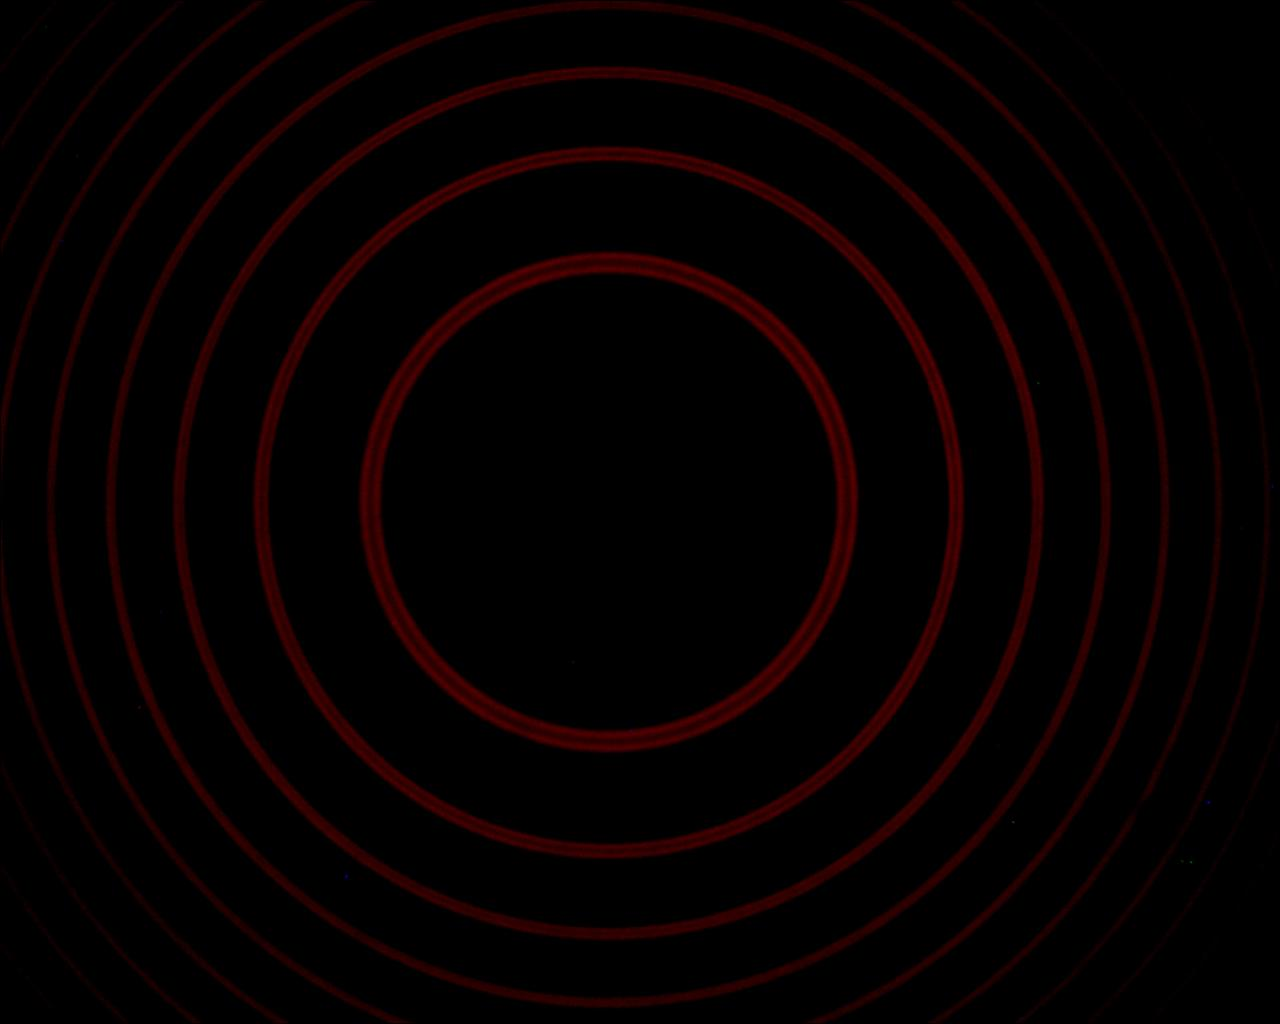
\includegraphics[width=8cm]{scripts/figs/ZEEMAN1A.jpg}\label{fig:zeeman_1A}}
    \subfloat[][$B = 2A$]{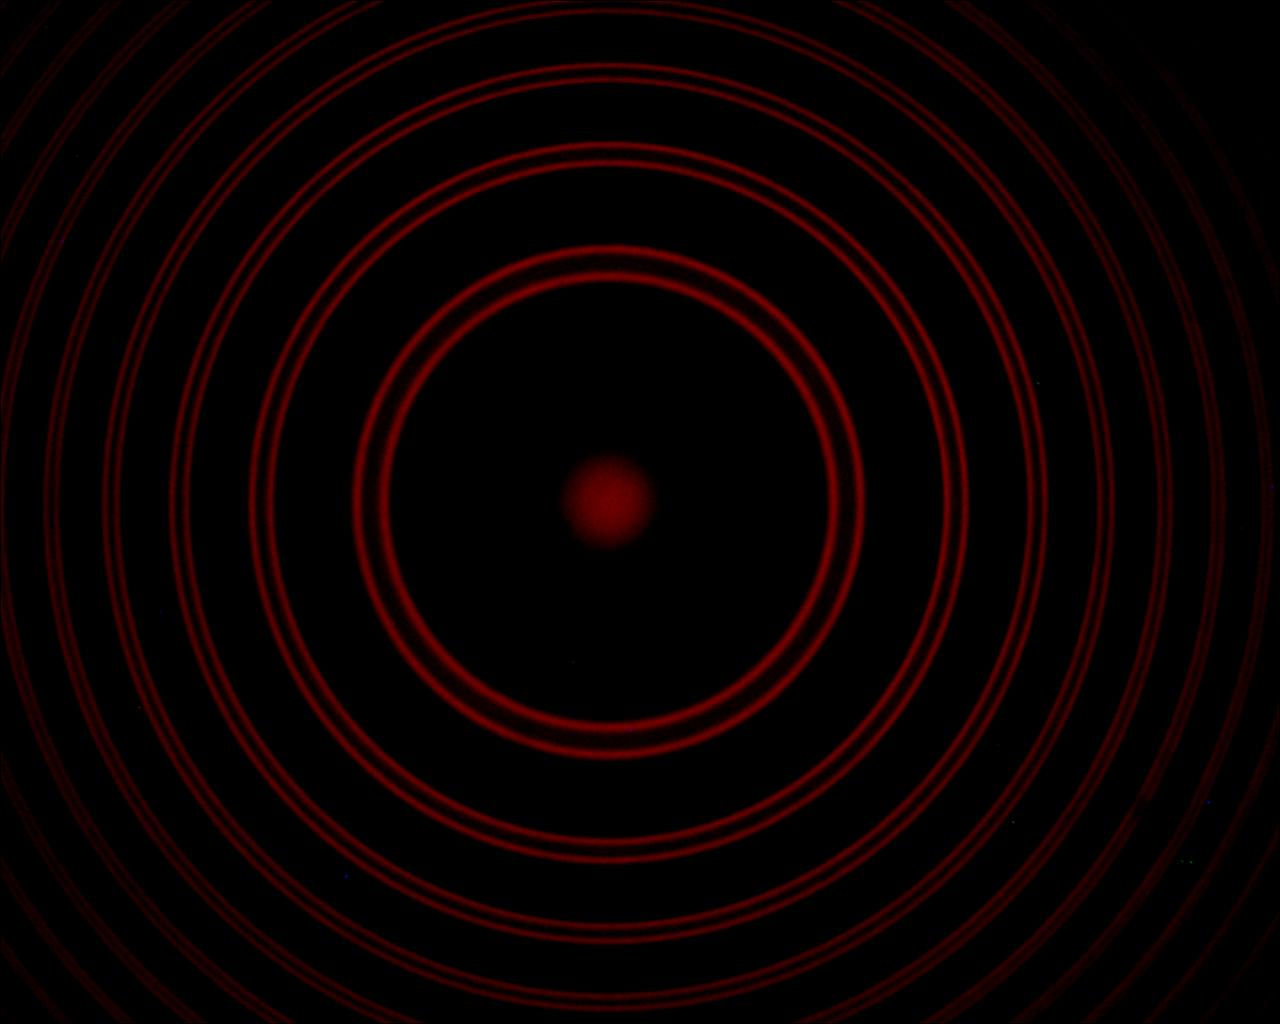
\includegraphics[width=8cm]{scripts/figs/ZEEMAN2A.jpg}\label{fig:zeeman_2A}} \\
    \subfloat[][$B = 3A$]{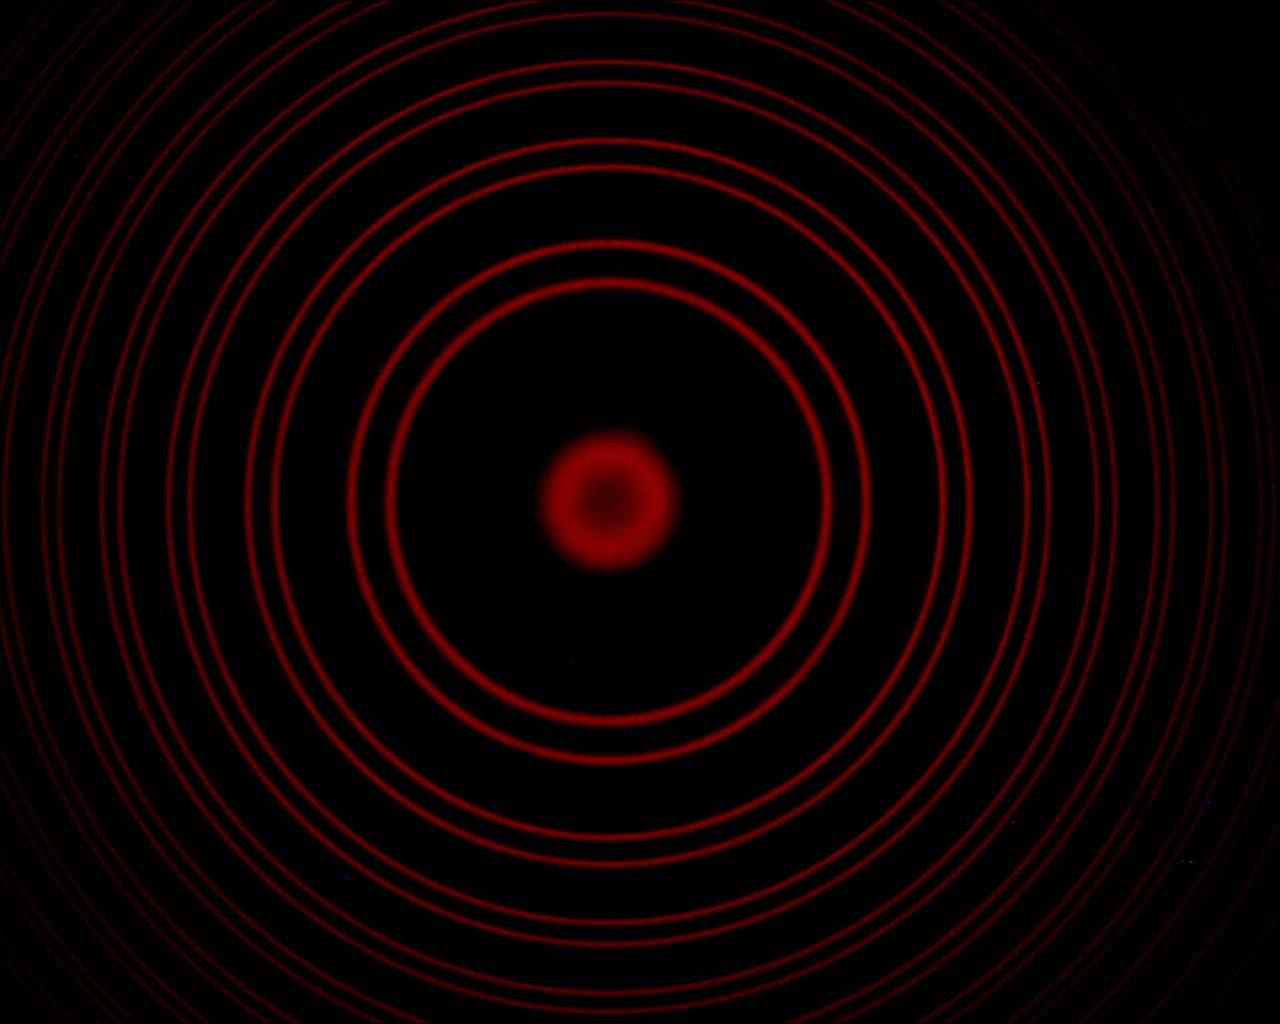
\includegraphics[width=8cm]{scripts/figs/ZEEMAN3A.jpg}\label{fig:zeeman_3A}}
    \subfloat[][$B = 4A$]{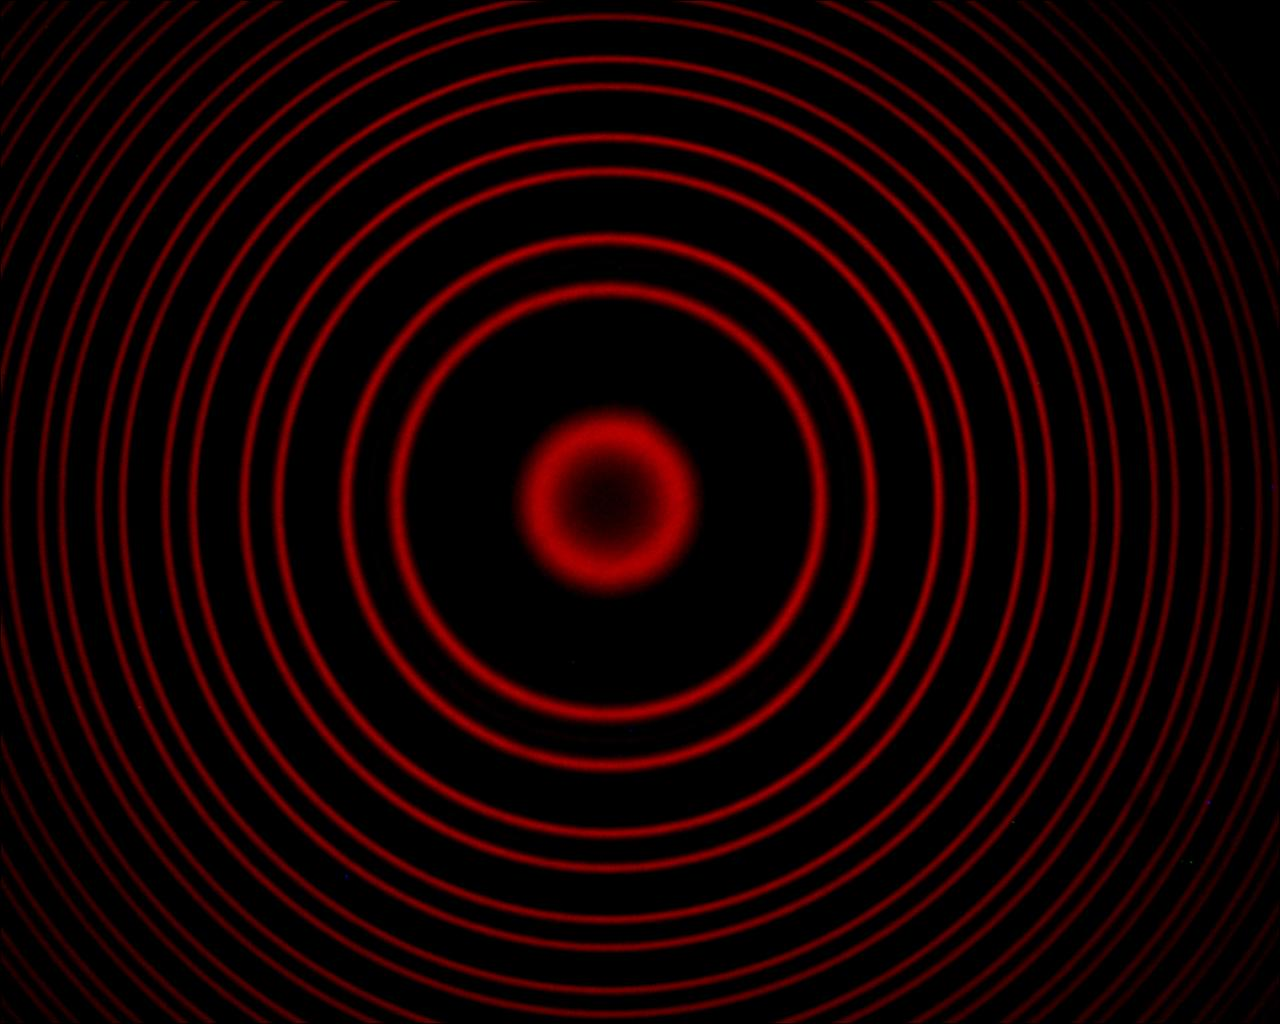
\includegraphics[width=8cm]{scripts/figs/ZEEMAN4A.jpg}\label{fig:zeeman_4A}}
    \caption{Observed difraction lines due to $\pi$-transitions for different magnetic fields}
    \label{fig:scale1}
  \end{figure}
  \twocolumn

\section{\label{sect:discuss}Discussion}

\section{\label{sect:conclusion}Conclusion}


\bibliographystyle{plain}
\bibliography{references.bib}

%%%%%%%%%%%%%%%%%%%%%%%%
%%% END OF MAIN BODY %%%
%%%%%%%%%%%%%%%%%%%%%%%%

%\appendix*
%\section{Scripts}
%\lstinputlisting[language=python]{scripts/lesVideo_conv.py}
%\lstinputlisting{scripts/data/labdata.dat}

\end{document}